%----------------------------------------------------------------------------
\chapter{Tervezés és megvalósítás}
%----------------------------------------------------------------------------

A projektet Visual Studio Code segítségével fejlesztettem, amely egy ingyenes és nyílt forráskódú fejlesztői környezet. Bár alapvetően könnyűsúlyú, ennek ellenére erőteljes szövegszerkesztő, mivel számos programozási nyelvet és technológiát támogat. A telepítése után nagyban testreszabhatjuk saját igényeink szerint és számos egyéb funkciókhoz juthatunk a bővítmények telepítésével.

6 részre bontottam a projektet: instance, cryptorithms, languages, static, templates, cryptorithm  (\ref{fig:fileStruct})

\begin{itemize}
	\item\textbf{Instance}:
Az instance mappában van eltárolva az adatbázis lokálisan, melynek modelje a models.py fájlban van definiálva.

	\item\textbf{Cryptorithms}:
A cryptorithms mappában levő fájlokban kerültek kivitelezésre és implementálásra a kriptográfiai rendszerek.

	\item\textbf{Languages}:
A nyelvekért felelős .json kiterjesztésű fájlok itt vannak tárolva, itt van egy meghatározott struktúrában lefordított tartalma az oldalnak.

	\item\textbf{Static}:
A static alatt a .css és .js fájlok kerültek létrehozásra, melyek rendre a weboldal dizájnért és a dinamikus felületért felelősek.

	\item\textbf{Templates}:
A template mappába kerültek az alap .html fájlok, amelyek a tartalom megjelenitéséért felelősek.

	\item\textbf{Cryptorithm}:
A fő mappa a Cryptorithm, amely magába foglalja az előbb említett részeket, valamint az API kéréseket és válaszokat, a szessziókezeléshez, a projekt inicializálásához szükséges fájlokat, továbbá az adatbázis adatmodelljét és a projektet indító main fájlt.

\end{itemize}

\begin{figure}[!h]
	\centering
	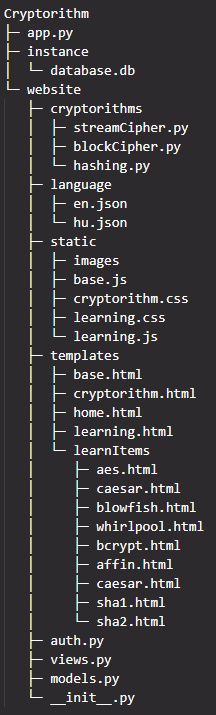
\includegraphics[scale=0.9]{images/fájlStruktúra}
	\caption{Rendszer fájl struktúrája}
	\label{fig:fileStruct}
\end{figure}

\section {Könyvtárak}
A következőekben bemutatom a jelentősebb Python könyvtárakat, melyek segítettek az alkalmazás implementálásában.

\begin{itemize}
  	\item\textbf{Cryptography:}
Kriptográfiai funkciókat és algoritmusokat kínál. Ez a könyvtár ideális választás a projektben, mivel számos kriptográfiai műveletet valósíthatunk meg vele. A Cryptography megbízható és jól dokumentált eszköz a kriptográfiai műveletek biztonságos végrehajtásához. Ennek a könyvtárnak a segítségével lett kivitelezve az AES rendszer.

 	 \item\textbf{Flask:}
A projektben a Flask keretrendszert használom a webes alkalmazás felépítéséhez és a kérések kezeléséhez. A Flask könnyen tanulható és rendkívül rugalmas, ami lehetővé tette, hogy könnyedén kialakítsam a vágyott funkciókat és testreszabhassam az alkalmazást.

A következő kódrészlet a tanulói oldal betöltésének kérését mutatja be:
\begin{lstlisting}[caption={Learning oldal renderelése}, captionpos=b, language = Python]
@views.route('/learning/<language>', methods=['GET', 'POST'])
def learning(language):
    if(language not in languages):
        language = app_language
    return render_template("learning.html", user=current_user, language=language, **languages[language])
\end{lstlisting}

 	 \item\textbf{FlaskSQLAlchemy:}
A FlaskSQLAlchemy egy könnyen használható és hatékony ORM (Object-Relational Mapping) könyvtár, amely lehetővé teszi az adatbázis műveletek kezelését a Flask alkalmazásban. Az SQLAlchemy révén a FlaskSQLAlchemy segít az adatbázis kapcsolatok kezelésében, az adatmodell osztályok definiálásában és az adatbázis műveletek végrehajtásában. A FlaskSQLAlchemy használata átlátható és hatékony adatbázis-interakciókat tesz lehetővé a projektben.

A következő kódrészlet az adatbázis modellek implementálását mutatja be:
\begin{lstlisting}[caption={Adatbázis modellek}, captionpos=b, language = Python]
class User(db.Model, UserMixin):
    id = db.Column(db.Integer, primary_key=True)
    email = db.Column(db.String(150), unique=True)
    password = db.Column(db.String(150))
    first_name = db.Column(db.String(150))
    datas = db.relationship('Data')

class Data(db.Model):
    id = db.Column(db.Integer, primary_key=True)
    data = db.Column(db.String(10000))
    cryptype = db.Column(db.String(100))
    paramA = db.Column(db.String(100), nullable=True)
    paramB = db.Column(db.String(100), nullable=True)
    user_id = db.Column(db.Integer, db.ForeignKey('user.id'))
\end{lstlisting}

\pagebreak
 	 \item\textbf{FlaskLogin:}
A FlaskLogin egy hasznos kiegészítő a Flask keretrendszerhez, amely segít az autentikáció és az azonosítás kezelésében a webes alkalmazásban. Ennek segítségével egyszerűen implementálhattam a felhasználói regisztrációt, bejelentkezést és kijelentkezést a rendszerben. Ez a könyvtár felelős a felhasználói munkamenetek és a hozzáférési jogosultságok kezeléséért.

A következő kódrészletek a flask login modulja egy szemléltetése a regisztrációra és kijelentkezésre:
\begin{lstlisting}[caption={Flask bejelentkezés kódrészlet}, captionpos=b, language = Python]
new_user = User(email=email, first_name=first_name, password=generate_password_hash(password1, method='sha256'))
db.session.add(new_user)
db.session.commit()
login_user(new_user, remember=True)
\end{lstlisting}

\begin{lstlisting}[caption={Flask kijelentkezés kódrészlet}, captionpos=b, language = Python]
@auth.route('/logout/<language>', methods=['GET'])
@login_required
def logout(language):
    logout_user()
    return redirect(url_for('auth.login', language=language))
\end{lstlisting}

 	 \item\textbf{Json:}
A JSON (JavaScript Object Notation) egy könnyen olvasható és írható adatformátum, amely széles körben használatos az adatok strukturált tárolására és átvitelére. A JSON könyvtárat használva a projektben könnyedén kezelhettem a JSON adatokat.

A alábbiakban látható a megvalósítás angol nyelvhez:
\begin{lstlisting}[caption={JSON angol kódrészlet}, captionpos=b]
"cryptorithm": {
    "login": "Login",
    "email": "Email",
    "password": "Password",
    "no_account": "Don't have an account?",
    "signup": "Sign Up",
    "already_account": "Already have an account?"
  }
\end{lstlisting}

\pagebreak
	 \item\textbf{Egyebek:}
Mindezekután szeretném megemlíteni azokat a könyvtárakat amelyek csak néhány művelet elvégzésére voltak igénybevéve, de ennek ellenére fontos részét képezik a rendszernek.
\begin{itemize}
 	 \item{Base64}
 	 \item{Glob}
 	 \item{Os}
 	 \item{Math}
 	 \item{Hashlib}
 	 \item{Random}
\end{itemize}
\end{itemize}


\section {Jinja2}
\label{sec:jinja2}
A Jinja2 egy erőteljes és rugalmas sablonmotor Python nyelvhez. Arra tervezték, hogy segítsen a dinamikus tartalmú weboldalak generálásában a sablonok és adatok kombinálásával. A Jinja2 a Flask keretrendszer alapértelmezett sablonmotorja, de függetlenül is használható más projektekben. Egyszerű és kifejező szintaxissal rendelkezik, amely hasonlít a HTML-hez, viszont tartalmaz kiegészítő jelöléseket és vezérlőstruktúrákat.

Fő alapvető jellemzője és funkciója amit használtam a következő:

 	 \textbf{Sablonok:}
Lehetővé teszi a HTML-szerű sablonok létrehozását, amelyekben helytartókat (placeholder) és vezérlőstruktúrákat használhatunk. A helytartók fogadják a dinamikus adatokat, amelyeket a sablonmotor behelyettesít az adott oldalra. Ezzel a funkcióval valósítottam meg, hogy a weboldal tartalma igény szerint idegen nyelvűek számára is használható legyen.
Az alábbi kód szemlélteti ennek használatát, ahol a dupla-kapcsos zárójelek közötti változók a Jinja2 elemei amelyeket a nekik megfelelő json fájlok tartalmával tölt fel:
\begin{lstlisting}[caption={Jinja2 sablon kódrészlet}, captionpos=b,  language = HTML]
<button type="submit" class="btn" value="login" name="submit_button">{{cryptorithm.login}}</button>
<div class="login-signup">
	<p>{{cryptorithm.no_account}}</p>
	<a href="#" class="signup-link">{{cryptorithm.signup}}</a>
</div>
\end{lstlisting}
